%!TEX root = main.tex

\section{Quality model of \name}
\label{sec:jnd}

We start with the quality model of \name, which estimates the subjective user experience for a given video content and real-time user action (viewpoint position and velocity).
%We begin with a brief introduction of the traditional video quality metric framework on which we build our model and how the new quality-determining factors can be incorporated (\S\ref{subsec:jnd:framework}), and then provide detailed empirical analysis on the impact of these new factors affect the perceived quality (\S\ref{subsec:jnd:details}).

\subsection{A general video quality framework}
\label{subsec:jnd:framework}

%\jc{need to tighten the text}

%It is defined based on Just-Noticeable-Distortion (JND) theory \cite{JND}. Given the original video frame and a compressed video frame, user can notice their difference only if the difference between them is above a visibility threshold. When the different is under this threshold, it will not detected by user. This threshold is called Just-Noticeable-Distortion.
%
%Based on JND theory, PSPNR is defined by accumulating error of each pixel which can be detected by user:

We first briefly introduce the framework on which we build our video quality metric that incorporates the new quality-determining factors. 
We use Peak Signal-to-Perceptible-Noise Ratio (PSPNR)~\cite{PSPNR}, a widely-used metric to measure perceived quality. 
It improves on the classic Peak Signal-to-Noise Ratio (PSNR) by taking into account only the changes perceptible by the viewer.
So images with the same level pixel-level quality distortion (\ie same PSNR) can have different PSPNR values, if users tend to be less sensitive to one image (\eg typically more complex or darker, etc) than another.

The key to PSPNR is the notion called Just-Noticeable Difference (JND)~\cite{??}, which is the minimal changes in pixel value that can be noticed by viewers. 
PSPNR can be expressed mathematically as following
\vspace{-0.3cm}
\begin{alignat}{2}\
\label{f1} PSPNR = 20 \times \log_{10}\frac{255}{\sqrt{PMSE}}
\end{alignat}
\vspace{-0.3cm}
\begin{alignat}{2}\
PMSE=\frac{1}{MN}\sum_{x,y}\left[ |p_{x,y} - \hat{p}_{x,y}| - JND_{x,y}\right]^2 \times \Delta (x, y)
\end{alignat}
\vspace{-0.3cm}
\begin{alignat}{2}\
\Delta (x, y) =\left\{
\begin{aligned}
1, & &|p_{x,y} - \hat{p}_{x,y}| > JND_{x,y} \\
0, & &|p_{x,y} - \hat{p}_{x,y}| \le JND_{x,y}
\end{aligned}
\right.
\end{alignat}
where $M,N$ denote the image size, $p_{x,y}$ and $\hat{p}_{x,y}$ pixel values at $(x, y)$ in original video frame and compressed video frame, and $JND_{x,y}$ the JND threshold at pixel $(x, y)$.

PSPNR helps to model the user-perceived quality of \vrvideos, because it wraps all factors other than pixel-level distortion in the abstraction of JND, effectively {\em separating} the their impact on the perceived quality from the impact of of pixel-level distortion. 
Traditionally, the notion of JND has been shown to be related to a series of factors: texture complexity~\cite{??}, content luminance~\cite{??}, viewpoint-object distance~\cite{??} and so forth.
Following this approach, we empirically found that it is possible to incorporate the three new quality-determining factors in the calculation of JND.



%Compared with PSNR (which is widely used in evaluating video / image quality), the core difference of PSPNR is introducing a term $JND(x, y)$ for each pixel $(x, y)$. So how to compute JND for each pixel $(x, y)$ is an important issue. We will present our JND computation in the following section.
%
%The just-noticeable distortion (JND) provides cues for measuring the visibility of the Human Vision System (HVS). JND refers to the maximum distortion which cannot be perceived by human. It describes the perceptual redundancy of the picture by providing the visibility threshold. The JND model generally exploits the visibility of the minimally perceptible distortion.
%
%JND has been well-studied in traditional video display since 1995. The most basic and solid research is about the relationship between content luminance and JND. \cite{luminance1}  and \cite{PSPNR} prove that content with moderate content luminance have low JND value, while content with very high or very low content luminance have high JND value. 

%In recent years, based on the insight of content luminance - JND relationship, researchers have explored some more factors which are also related to JND, such as texture complexity, viewpoint-object distance (\cite{PSPNR}, \cite{distance}) and some other factors. Although the relationship between multiple JND factors may be complex, for simplicity, we can decouple them into several single factors. For example, \cite{distance} set up a user study to test the JND value with the combined effect of content luminance and viewpoint-object distance. The result proves that viewpoint-object distance can be considered independently from content luminance. It can be regarded as a coefficient which can be directly multiplied on JND value computed by content luminance. Based on this insight, JND computation for multiple factors is decoupled into several single factors. This significantly simplify the JND computation.

%\subsection{JND for \vr videos}

%
%
%In VR display, user experience is very different because 3 new factors should be taken into consideration: (1) viewpoint moving decreases visual acuity, (2) low Depth-of-Field decreases visual acuity and (3) light / dark adaptation decreases visual acuity. So previous JND model for traditional video display can not be directly applied on VR video display. Moreover, it is unknown that (1) how these new factors influence JND with combined effect of old factors, and (2) if they can also be decoupled into several single factors, like viewpoint-object distance \cite{distance}.
%
%Strictly answering these 2 questions needs to test JND value for each possible combinations of all factors (including all possible luminance, texture, viewpoint-object distance, viewpoint moving speed, Depth-of-Field and light / dark adaptation, which make up a 6-dimension feature space), which is not practical for a real-world user study. For simplicity, we imitate the user study in \cite{distance}, which makes only 2 factors variable and other 4 factors fixed, then we can know how is the combined effect of the 2 factors to JND, and if they can be decoupled to 2 single factors which independently influence JND.
%
%So we present 3 user studies: (1) JND v.s. luminance \& viewpoint moving speed. (2) JND v.s. luminance \& depth of field. (3) JND v.s. luminance \& light / dark adaptation. We evaluate the effect of 3 VR-only factors to JND, each with combined effect of luminance, since luminance is the most well-studied JND factor.
%
%We conduct the user study using real Head Mounted Device (HMD). Parameters of proposed HMD are listed as Table \ref{table1}:
%
%\begin{table}[h]
%\centering
%\caption{HMD Parameters}\label{table1}
%\begin{tabular}{|p{3.5cm}|p{3.5cm}|}
%\hline
%Equipment & Oculus GO\\
%CPU & Xiaolong 821 customized drive Edition\\
%Memory & 3GB\\
%Screen Resolution & 2560 $\times$ 1440\\
%Refresh Rate & 72Hz\\
%Fixed pupil distance & 63.5mm\\
%\hline
%\end{tabular}
%\end{table}
%
%X subjects participated in the experiments, including X males and X females. All of them were in their twenties. The subjects obtained extensive practice during the experiments.
%
%In this paper, we imitate the human visibility experiments in \cite{PSPNR}. In the experiment, a small square area, 32 x 32 pixels, is located in the center of a flat field of constant grey level (luminance). For each possible grey level (luminance) of the square area, the noises of fixed amplitude are randomly added to or subtracted from the pixels within the square area. Through varying the amplitude of the noise, the visibility threshold for each grey level is determined when the square region contaminated by the noises is just noticeable. 
%

\subsection{Profiling \vrjnd}
\label{subsec:jnd:details}

We call the new JND model that takes as input the three new quality-determining factors, \vrjnd.
Conceptually, other than the traditional factors (texture complexity, content luminance, and viewpoint-object distance), the \vrjnd threshold of a pixel $(x,y)$ (which is part of an object $O$) is calculated given the following information: the speed of $O$ relative to the viewpoint speed, the luminance of $O$ relative to where the viewpoint focused on a few seconds ago, and the DoF difference between $O$ and the viewpoint focused object. 


\mypara{Methodology}
We empirical build the correlation between these factors and \vrjnd based on an IRB-based user study.
\jc{add a short description of the evaluation setup, value range of each parameter, default value of each parameter when varying one or more control variables, etc}

\mypara{Impact of single factors}
\jc{briefly explain each of the subgraphs in Figure~\ref{fig:single-factor} and what the correlation looks like (non-linearity? non-monotonicity? any suprising trend?)}

\begin{figure}
  \centering
  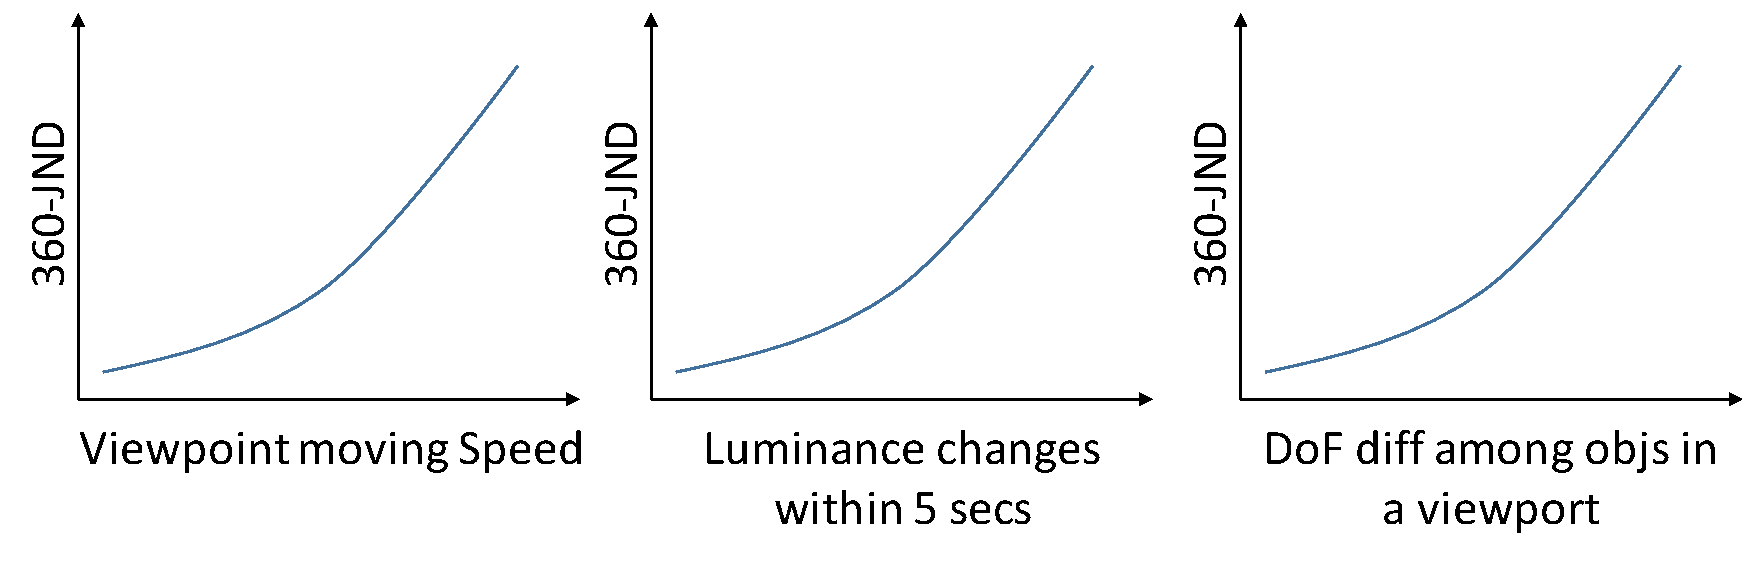
\includegraphics[width=0.5\textwidth]{figures/single-factor.pdf}
  \caption{Single-factor analysis. The impact of each of the three factors on \vrjnd.}
  \label{fig:single-factor}
 \end{figure}

\mypara{Impact of multiple factors}
\jc{briefly explain the impact of any two factors on \vrjnd, shown in Figure~\ref{fig:two-factor}. how does the graph show the correlations are mutually independent? also mention such mutual independence has been observed in traditional jnd studies}

\begin{figure}
  \centering
  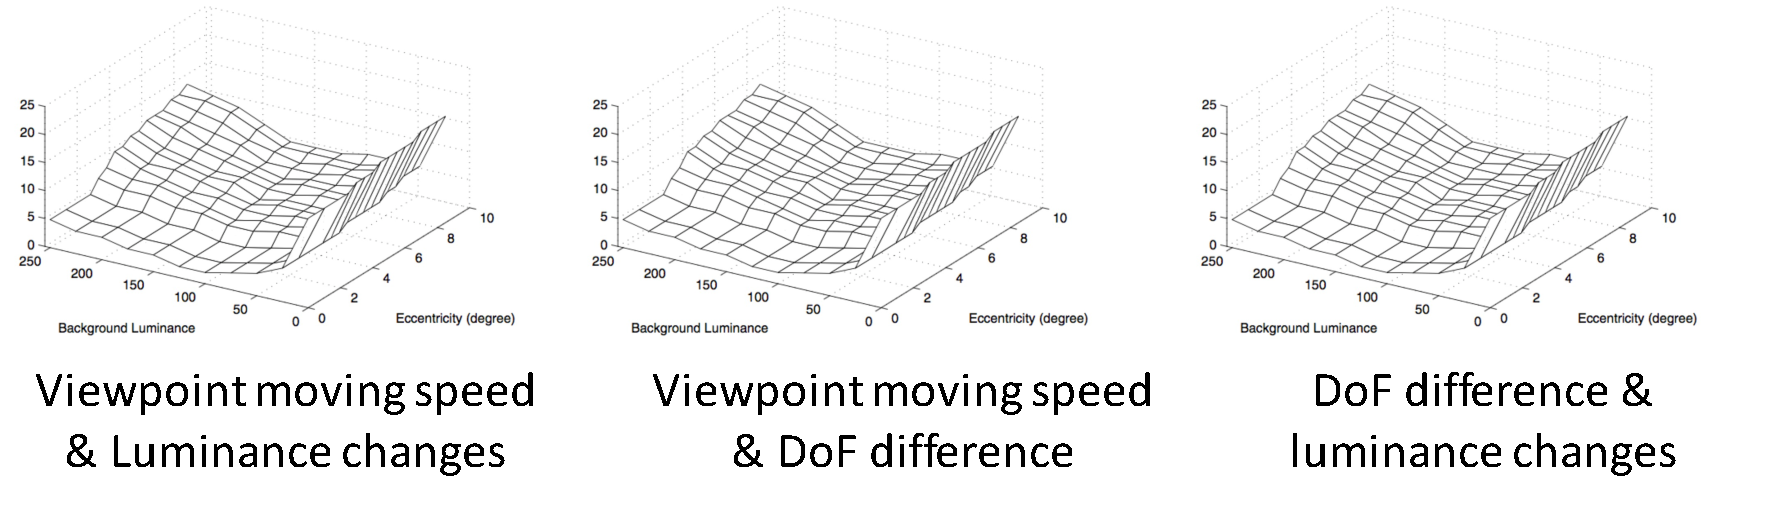
\includegraphics[width=0.5\textwidth]{figures/two-factor.pdf}
  \caption{Multi-factor analysis. The impact of two factors on \vrjnd appear to be largely mutually independent.}
  \label{fig:two-factor}
 \end{figure}
 
\mypara{Interaction with existing JND model}
In addition, we also vary traditional JND values while changing one of the three new factors, and found their impact on \vrjnd is also largely independent to the existing JND factors.
\jc{do a similar analysis between traditional jnd and the new factors. no need the show the figures, if not enough space}

\mypara{Putting it together}
\jc{give the complete equation of \vrjnd, and the parameters as much as possible}

\mypara{Validation with opinion score}
\jc{explain Figure~\ref{fig:pspnr-accuracy}}.

\begin{figure}
  \centering
  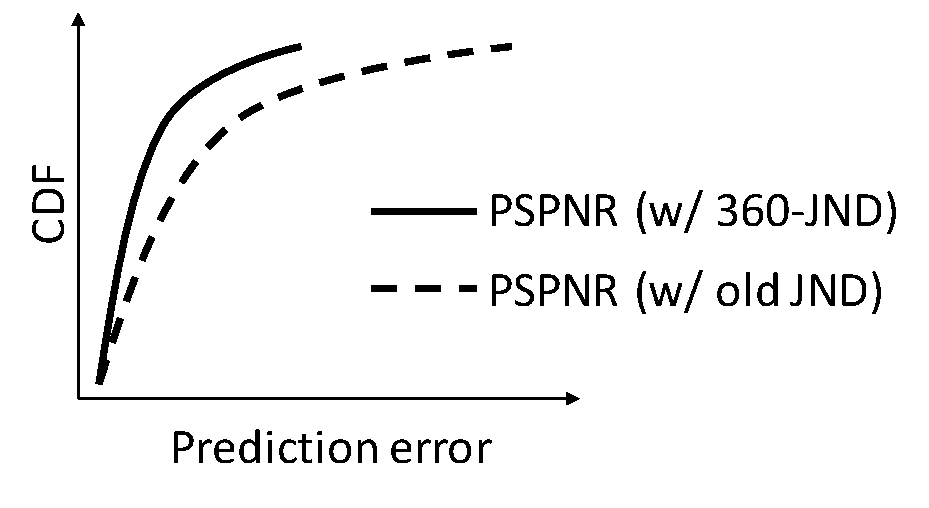
\includegraphics[width=0.5\textwidth]{figures/pspnr-accuracy.pdf}
  \caption{PSPNR with the proposed \vrjnd can predict user rating more accurately than the  existing PSPNR metric.}
  \label{fig:pspnr-accuracy}
 \end{figure}

Lastly, this in no way provides a complete list of quality-determining factors. 
Rather, it provides a systematic methodology to incorporate future factors in the same framework of \vrvideo quality metrics.

%\begin{figure}
%  \centering
%  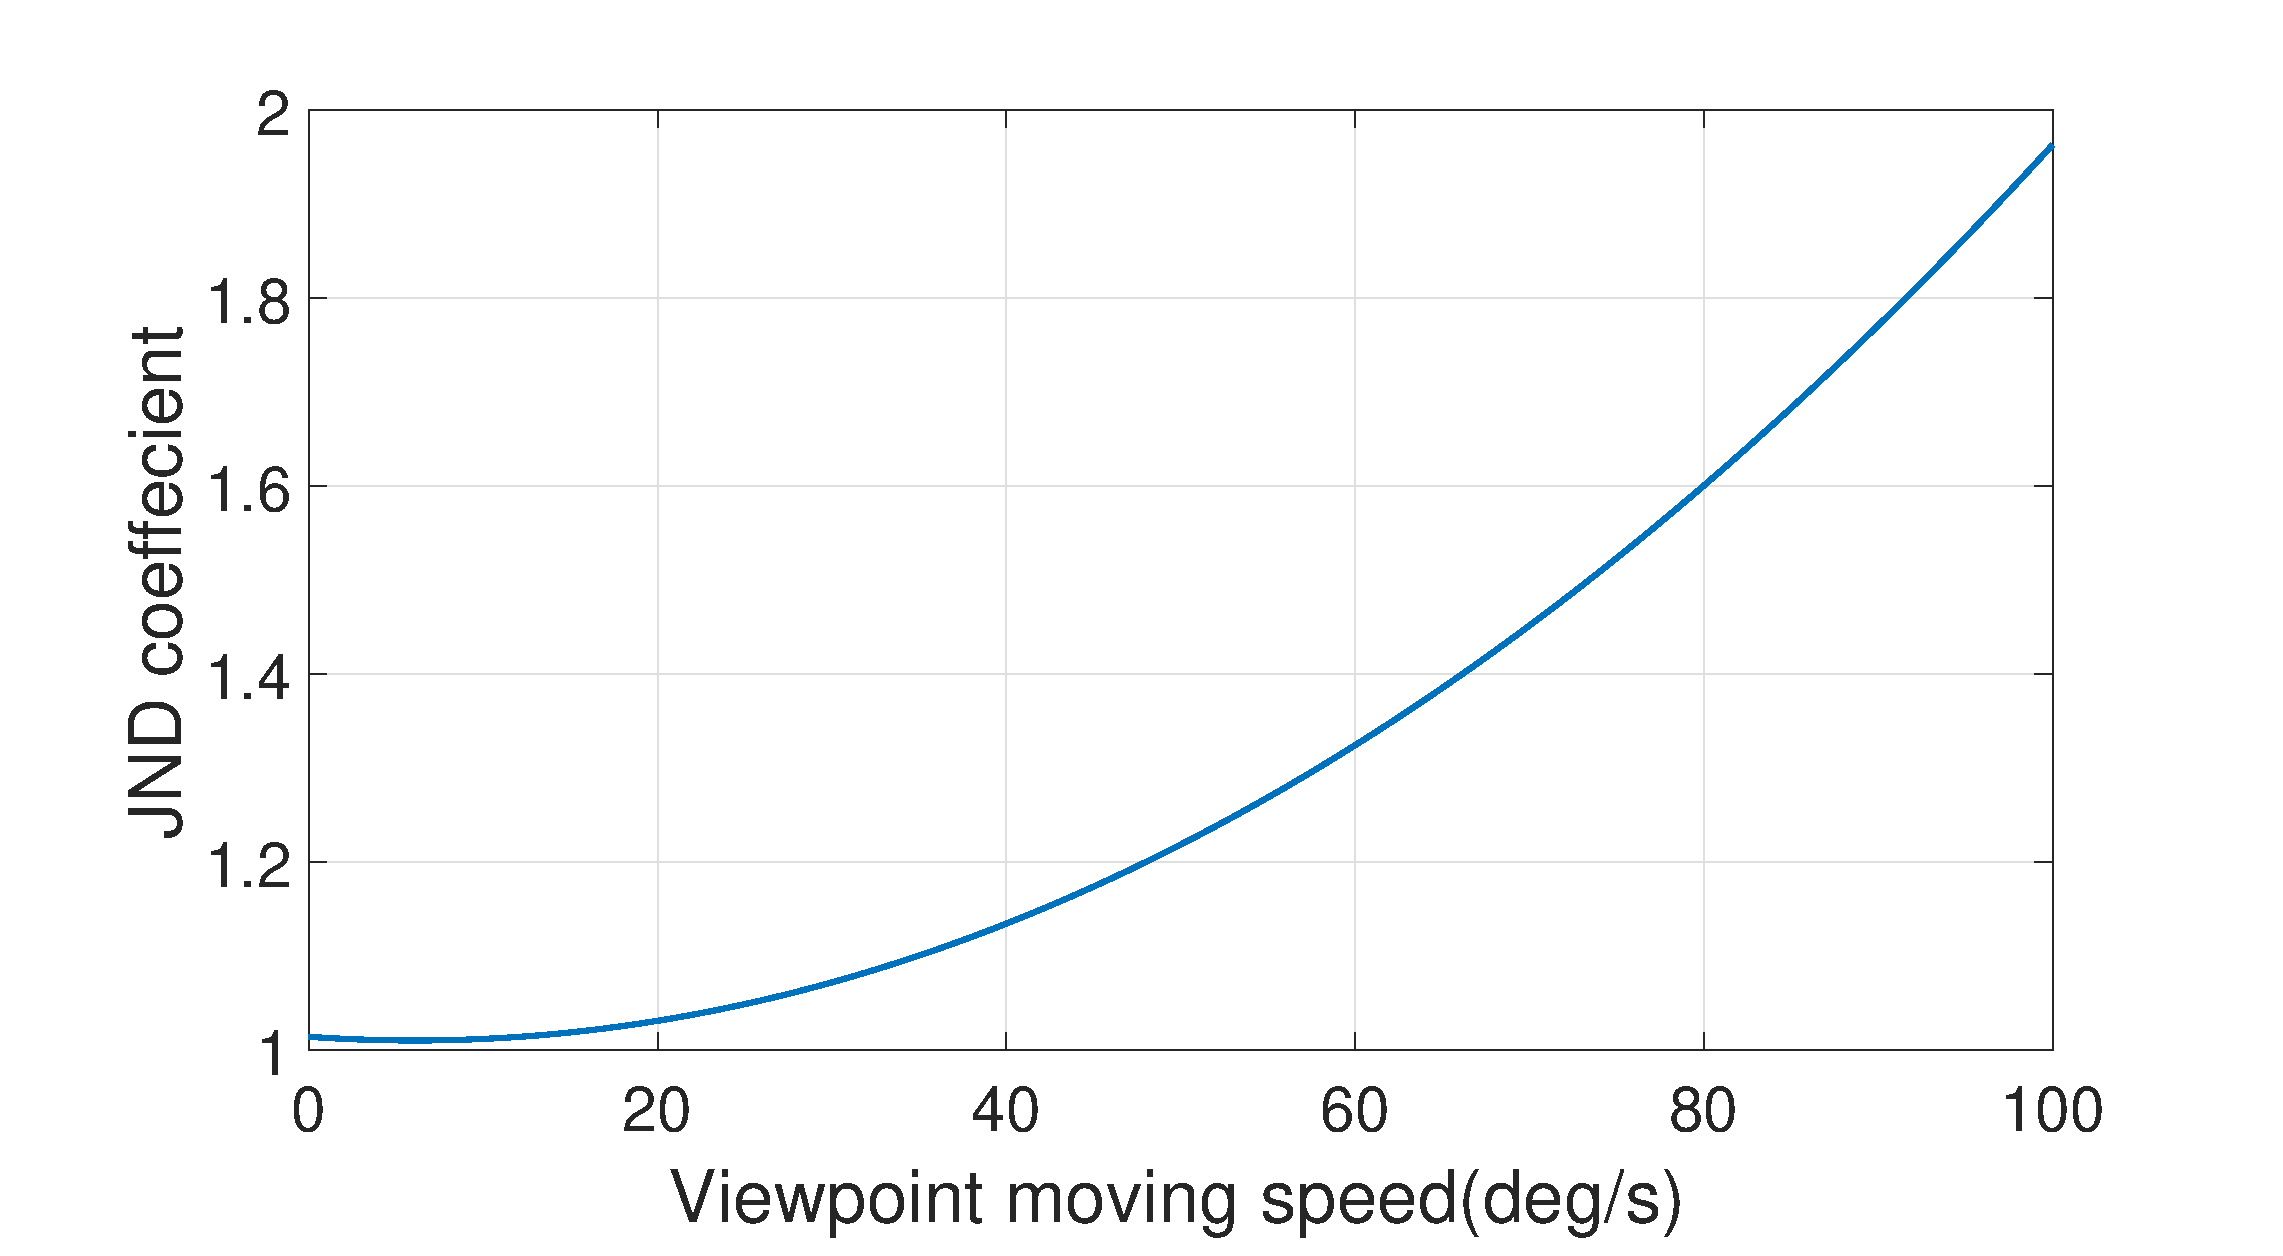
\includegraphics[width=2.5in]{images/JNDspeed.eps}
%  \caption{$f_{track}(v)$, the JND coefficient of viewpoint moving speed.}
%  \label{JNDspeed-track}
%  \end{figure}







